\chapter*{不定积分每日一题}

\refer{《积分的方法与技巧》金玉明\ 顾新身\ 毛瑞庭\ /\ 编著}

\exercise{求积分$\int{\sqrt{x^2-4}\d x}$}

\teacher{夏明宇}

\postdate{2022年12月8日}

\result{\frac{1}{2}x^2\sqrt{x^2-4}-\ln{\qty(x+\sqrt{x^2-r})}^2+C}

\analysis{对于$\int{\sqrt{x^2-a^2}\d x}$及其类似的积分，可采用三角替代法，利用直角三角形的边、角与三角函数的关系进行换元以简化计算.}

\solution{
  看到$\sqrt{x^2-a^2}$后，很容易想到直角三角形中三条边所满足的勾股定理，即$x$为斜边长度，$a$为其中的一条直角边长度，$\sqrt{x^2-a^2}$为另一条直角边长度，这时就可利用三条 边的三角函数关系进行换元.
  \begin{center}
    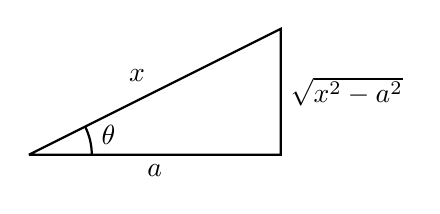
\begin{tikzpicture}[scale=0.8]
        \draw [thick] (0,0)--(4,0)--(4,2)--(0,0);
        \node [anchor=west] at (4,1) {$\sqrt{x^2-a^2}$};
        \node [anchor=north] at (2,0) {$a$};
        \draw [thick] (1,0) arc (0:26.565:1);
        \node [anchor=south west] at (1,0) {$\theta$};
        \node [anchor=south east] at (2,1) {$x$};
    \end{tikzpicture}
  \end{center}

    如图，设直角边$a$与斜边$x$之间的夹角为$\theta$，则有
    \formula{x=a\sec{\theta},\ \sqrt{x^2-a^2}=a\tan\theta,\ \d x=a\sec{\theta}\tan{\theta}\d\theta}
    那么关于$x$的积分就变成了关于$\theta$的积分，即
    \formula{
        \addtolength{\jot}{-0.5em}
        \begin{aligned}
            \int{\sqrt{x^2-a^2}\d x}&=\int{a\tan{\theta}\cdot a\sec{\theta}\tan{\theta}\d\theta}\\
            &=a^2\int{\sec{\theta}\tan^2{\theta}\d\theta}\\
            &=a^2\int{\sec{\theta}\qty(\sec^2{\theta}-1)\d\theta}\\
            &=a^2\int{\sec^3{\theta}\d\theta}-a^2\int{\sec{\theta}\d\theta}
        \end{aligned}
    }
    那么剩下就变成了求$\int{\sec{\theta}\d\theta}$和$\int{\sec^3{\theta}\d\theta}$.


    这俩个都可以用\hypertarget{12.8}{上下同乘同除$\sin{\theta}$或$\cos{\theta}$的操作转化为有理分式积分}
    \formula{\int{\sec{\theta}\d\theta}=\int{\frac{\d\theta}{\cos{\theta}}}=\int{\frac{\cos{\theta}\d\theta}{\cos^2{\theta}}}=\int{\frac{\d\sin{\theta}}{1-\sin^2{\theta}}}}
    \formula{\int{\sec^3{\theta}\d\theta}=\int{\frac{\cos{\theta}\d\theta}{\cos^4{\theta}}}=\int{\frac{\d\sin{\theta}}{\qty(1-\sin^2{\theta})^2}}}


    或者用下面这两种方式也可以：
    \formula{
        \begin{aligned}
            \int{\sec{\theta}\d\theta}&=\int{\frac{\d\theta}{\cos{\theta}}}=\int{\frac{\d\qty(\theta+\dfrac{\pi}{2})}{\sin{\qty(\theta+\dfrac{\pi}{2})}}}=\int{\frac{\d\qty(\theta+\dfrac{\pi}{2})}{2\sin{\qty(\theta+\dfrac{\pi}{4})\cos\qty({\theta+\dfrac{\pi}{4}})}}}\\
            &=\int{\frac{\d\qty(\dfrac{\theta}{2}+\dfrac{\pi}{4})/\cos^2{\qty(\dfrac{\theta}{2}+\dfrac{\pi}{4})}}{\sin{\qty(\dfrac{\theta}{2}+\dfrac{\pi}{4})}/\cos{\qty(\dfrac{\theta}{2}+\dfrac{\pi}{4})}}}=\int{\frac{\d\tan{\qty(\frac{\theta}{2}+\frac{\pi}{4})}}{\tan{\qty(\frac{\theta}{2}+\frac{\pi}{4})}}}\\
            &=\ln{\abs{\tan{\qty(\frac{\theta}{2}+\frac{\pi}{4})}}}+C\\
            \int{\sec^3{\theta}\d\theta}&=\int{\sec{\theta\d\sec{\theta}}}\\
            &=\sec{\theta}\tan{\theta}-\int{\tan{\theta}\d\sec{\theta}}\\
            &=\sec{\theta}\tan{\theta}-\int{\tan{\theta}\sec{\theta}\tan{\theta}\d\theta}\\
            &=\sec{\theta}\tan{\theta}-\int{\tan^2{\theta}\sec{\theta}\d\theta}\\
            &=\sec{\theta}\tan{\theta}-\int{\sec{\theta}\qty(\sec^2{\theta}-1)\d\theta}\\
            &=\sec{\theta}\tan{\theta}-\int{\sec^3{\theta}\d\theta}+\int{\sec{\theta}\d\theta}
        \end{aligned}
    }
        因此可得
        \formula{\int{\sec^3{\theta}\d\theta}=\frac{1}{2}\qty[\sec{\theta}\tan{\theta}+\ln{\abs{\tan{\qty(\frac{\theta}{2}+\frac{\pi}{4})}}}]+C}
        那么回到前面的积分，将上述结果代入则有：
        \formula{
            \begin{aligned}
                \int{\sqrt{x^2-a^2}\d x}&=\frac{a^2}{2}\sec{\theta}\tan{\theta}+\frac{a^2}{2}\ln{\abs{\tan{\qty(\frac{\theta}{2}+\frac{\pi}{4})}}}-a^2\ln{\abs{\tan{\qty(\frac{\theta}{2}+\frac{\pi}{4})}}}+C\\
                &=\frac{1}{2}a\sec{\theta}\cdot a\tan{\theta}-\frac{a^2}{2}\ln{\abs{\tan{\qty(\frac{\theta}{2}+\frac{\pi}{4})}}}+C\\
                &=\frac{1}{2}\qty(x\sqrt{x^2-a^2}-a^2\ln\abs{x+\sqrt{x^2-a^2}})+C
            \end{aligned}
        }
        这里利用了$a\tan{\qty(\frac{\theta}{2}+\frac{\pi}{4})=x+\sqrt{x^2-a^2}}$，证明如下：


        令$x=a\sec{\theta},\ \sqrt{x^2-a^2}=a\tan{\theta}$，因此有
        \formula{x+\sqrt{x^2-a^2}=a\sec{\theta}+a\tan{\theta}=a\qty(\frac{1}{\cos{\theta}}+\frac{\sin{\theta}}{\cos{\theta}})=a\frac{1+\sin{\theta}}{\cos{\theta}}}
        另一方面
        \formula{
            \begin{aligned}
                \tan{\qty(\frac{\theta}{2}+\frac{\pi}{4})}&=\frac{\tan{\dfrac{\theta}{2}}+\tan{\dfrac{\pi}{4}}}{1-\tan{\dfrac{\theta}{2}}\tan{\dfrac{\pi}{4}}}=\frac{1+\tan{\dfrac{\theta}{2}}}{1-\tan{\dfrac{\theta}{2}}}=\frac{\cos{\dfrac{\theta}{2}}+\sin{\dfrac{\theta}{2}}}{\cos{\dfrac{\theta}{2}}-\sin{\dfrac{\theta}{2}}}\\
                &=\frac{\sqrt{1+\cos{\theta}}+\sqrt{1-\cos{\theta}}}{\sqrt{1+\cos{\theta}}-\sqrt{1-\cos{\theta}}}=\frac{\qty(\sqrt{1+\cos{\theta}}+\sqrt{1-\cos{\theta}})^2}{2\cos{\theta}}\\
                &=\frac{2+2\sin{\theta}}{2\cos{\theta}}=\frac{1+\sin{\theta}}{\cos{\theta}}
            \end{aligned}
        }
        因此证明了
        \formula{x+\sqrt{x^2-a^2}=a\tan{\qty(\frac{\theta}{2}+\frac{\pi}{4})}}
        那么$a=2$的情况也是一模一样的操作，结果如下：
        \formula{\frac{1}{2}x\sqrt{x^2-4}-\ln{\qty(x+\sqrt{x^2-4})}}
}